
\section{Introduction}
%
CISM, the Community Ice Sheet Model, originates from the Glimmer\footnote{{\it Glimmer} was originally an acronym, reflecting the project's origin within the GENIE climate model. The meaning of the Glimmer acronym is no longer important but reflects the current codes origins within the original Glimmer project.}-CISM project. The evolution of the name towards its current form reflects the project's evolution from a stand-alone ice sheet model to a fully supported, coupled component of the \href{http://www2.cesm.ucar.edu/}{Community Earth System Model}, or CESM. CISM is a numerical model - a collection of software libraries, utilities and drivers  - used to simulate ice sheet evolution. CISM is modular in design and coded almost entirely in standards-complient Fortran 95. It currently supports two different ``dynamical cores", which solve the equations for the conservation of mass, energy, and momentum. As with previous versions of Glimmer and Glimmer-CISM, the current version of CISM supports a serial, shallow-ice representation of ice dynamics. New with CISM is support for ``higher-order" ice dynamics, scalable parallelism, and software links for coupling to modern, robust, C++ based, third-party solver libraries. 
%
\section{Overview}
%
Glimmer-CISM consists of several components:
%
\begin{itemize}

\item {\bf CISM\_DRIVER:} The high level driver code (i.e., the executable) that is used to run the ice sheet model. Unlike previous version of Glimmer and Glimmer-CISM, CISM\_DRIVER is used
for running the code in all model configurations (e.g., for idealized test cases with simplified climate forcing and for model runs based on realistic geometries and climate forcing data).  

%\item {\bf GLIDE:} {\bf G}eneral {\bf L}and {\bf I}ce {\bf D}ynamic {\bf E}lements: the dynamical core for the model based on shallow-ice dynamics. 
\item {\bf GLIDE:} The model dynamical core based on shallow-ice dynamics. This component is responsible for solving the governing conservation equations and determining ice velocities, internal ice temperature distribution, and ice geometry evolution (see Chapter \ref{ch:glide}). Aside from very minor changes, this is the same shallow-ice dynamical core used by previous versions of Glimmer and Glimmer-CISM. \textbf{SP: I think the following sentences need to be re-written or removed. I suggest we remove it and add a separate section below to discuss available options for climate forcing. Matt - this could include a description of the new code you added to allow for forcing via data SMB, etc.} In addition, GLIDE components determine isostatic adjustment and meltwater production. GLIDE needs some representation of the climate to run, provided by a {\it driver} program. The user may write their own driver code, or may use one of the four supplied drivers (see section \ref{subsec:climdrive}). 

\item {\bf GLISSADE:} The model dynamical core based on the 1st-order accurate Stokes approximation. As with GLIDE, this component is responsible for solving the governing conservation equations. Unlike GLIDE, GLISSADE is fully parallel in order to take advantage of modern, multi-processor, high-performance architectures (see Chapter \ref{ch:glissade}).

%\item {\bf GLINT:} {\bf GL}IMMER {\bf Int}erface. Originally developed for the GENIE %\footnote{Grid-ENabled Integrated Earth-system model} 
%Earth Systems Model, GLINT allows the core ice model to be coupled to a variety of global climate models, or indeed any source of time-varying climate data on a lat-long grid. 
\item {\bf GLINT:} GLINT allows the core ice model to be coupled to a variety of global climate models, or indeed any source of time-varying climate data on a lat-long grid. \textbf{SP: Do we need to add some documentation for Glint somewhere? Currently, I think all that we have is the Glint example test case.}

\item {bf Test Cases:} Idealized test cases, for both the GLIDE and GLISSADE dynamical cores and for the GLINT coupler. These are used to (1) confirm that the model is working as expected and (2) provide a range of simple model configurations from which new users can learn about model configuration options and start to construct their own configurations (see Chapter \ref{ch:tests}). 

\item {\bf Shared Code:} This includes a number of modules used regularly by all parts of the code. Examples include modules for declaring derived types, physical constants, and model parameters, and modules that handle parsing of the configuration file and data input / output (``i/o"), as discussed below.

\item {\bf Simple climate drivers:} Drivers that implement the experiments of the first phase of the EISMINT project, with idealised geometry. \textbf{SP: I don't know if we need this anymore. Probably falls under tests and / or GLINT or the section below? Since all of these tests now use CISM\_DRIVER, I think this is no longer needed / accurate.}

%% SP: commented out the remainder, since we aren't supporting these anymore (and GLUM is included above, w/o the silly name)
%\item {\bf EIS:} {\bf E}dinburgh {\bf I}ce {\bf S}heet climate driver based on a parameterisation of the equilibrium line altitude, sea-level surface temperatures and eustatic sea-level change. \textbf{SP: Not used/supported anymore - remove?}
%\item {\bf EISMINT3:} An implementation of a later part of the EISMINT project, concerning the modelling of the Greenland ice sheet. 
%\item {\bf GLUM:} {\bf G}Limmer {\bf U}seful {\bf M}odules, various utility procedures used by the other components. 
%\item Visualisation programs using GMT\footnote{Generic Mapping Tools}. 
\end{itemize}
%
%\begin{figure}[htbp]
%  \centering
%  \includegraphics[width=0.6\textwidth]{\dir/figs/Glimmer.eps}
%  \caption{Relationship between the various Glimmer components.}
%  \label{ug.fig.Glimmer}
%\end{figure}

%The relationship between the Glimmer components is illustrated in Figure \ref{ug.fig.Glimmer}. 
%
\subsection{Climate Drivers}
\label{subsec:climdrive}
\textbf{SP: Matt, can you take a stab at correcting / updating this section? Maybe we don't even need it anymore since we aren't really supporting most of the old climate drivers?}
The core ice sheet model, GLIDE, is connected to the climate via the surface mass balance and temperature fields and (optionally) a scalar value for eustatic sea level. These drivers can be derived from simple assumptions, e.g. uniform mass balance or EISMINT tests, or from climate model output, e.g. GENIE or a regional climate model. These components, and how they relate to each other, are outlined in Figure \ref{ug.glide}.
%
%\begin{figure}[htbp]
% \begin{center}
%   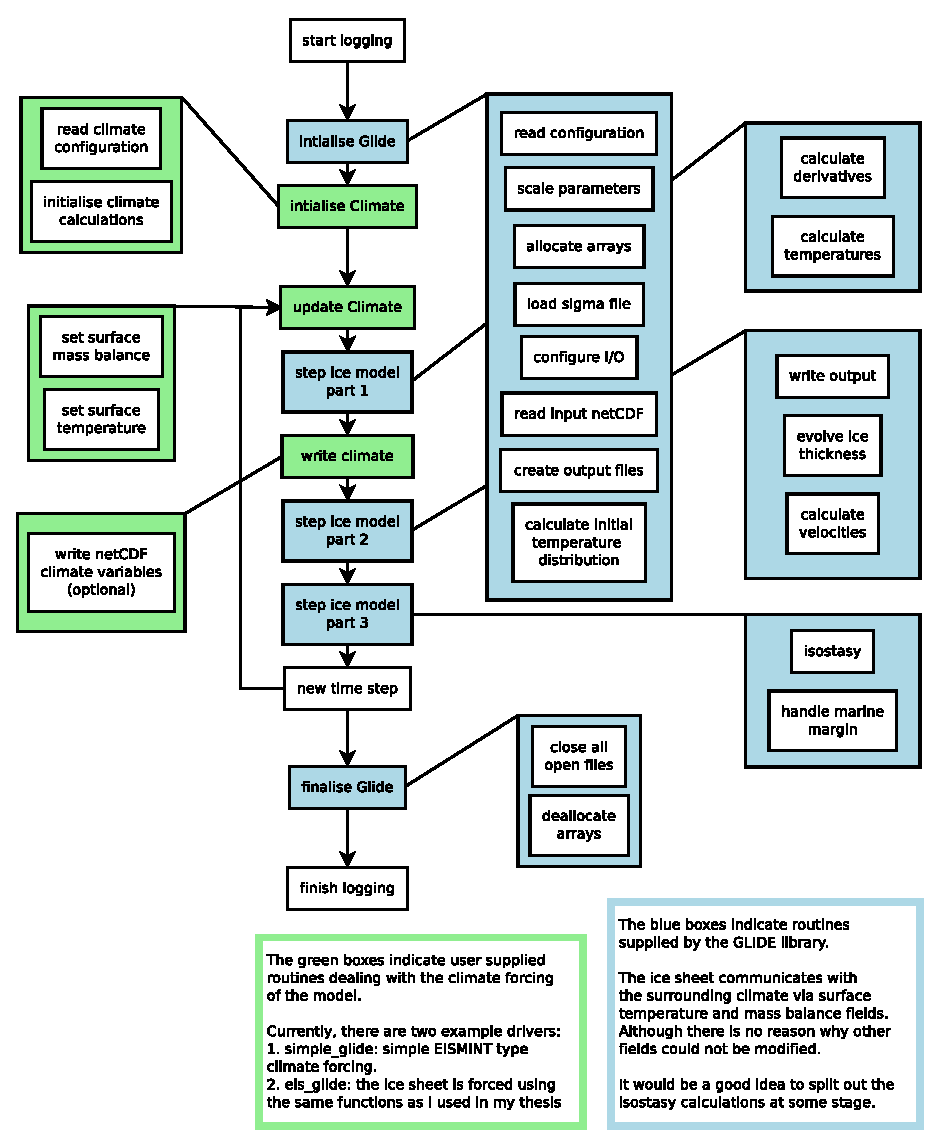
\includegraphics[width=0.9\textwidth]{\dir/figs/glide.eps}
% \end{center}
% \caption{Outline of the GLIDE and Climate components.}
%\label{ug.glide}
%\end{figure}
%
\subsection{Model Configuration, I/O and Visualisation}
In general terms, each component is configured using a configuration file similar to Windows \texttt{.ini} files. At run-time, model configuration is printed to a log file. 

2D and 3D data is read/written from/to NetCDF files using the CF (Climate-Forecast) metadata convention\footnote{\texttt{http://www.cgd.ucar.edu/cms/eaton/cf-metadata/}}. NetCDF is a scientific data format for storing multidimensional data in a platform- and language-independent binary format. The CF conventions specify the metadata used to describe the file contents.

Many programs can process and visualize NetCDF data, e.g. OpenDX, Matlab, IDL, etc. In section \ref{sec:install-netcdf} we provide installation instructions for a simple set of tools for manipulating and visualizing NetCDF data files. The following chapter discusses these and other software environment requirements in more detail.  
%Additionally, the Glimmer code bundle contains GMT scripts written in Python to visualise the output.

